\chapter{Ecuación del calor}
\label{cap:heat}
\begin{resumen}
	En este capítulo desarrollaremos dos métodos numéricos, basados en las diferencias finitas, para aproximar la solución a la ecuación del calor en una  y dos dimensiones.
\end{resumen}

\section{Caso lineal}
En el caso unidimensional, la ecuación del calor es de la forma

\begin{equation}
	\frac{\partial u}{\partial t} = \frac{\partial ^2u}{\partial x^2}
\end{equation}

La condición que pediremos para asegurar la existencia y unicidad de la solución será tener un valor concreto en el tiempo inicial ($t=0$) y conocer el valor de la solución a lo largo de la frontera del intervalo, por lo que el problema queda de la siguiente manera
\begin{equation}\label{eq:1dheat}
	\begin{cases} 
		\frac{\partial u}{\partial t}(x,t) = \frac{\partial ^2u}{\partial x^2}(x,t), & a\leq x\leq b, \hspace{5px} 0\leq t \leq T,\\
		u(x,0)=f(x), & a\leq x\leq b, \\
		u(a,t)=\alpha(t), & 0<t,\\
		u(b,t)=\beta(t), & 0<t.
	\end{cases}
\end{equation}


Salta a la vista que el dominio de este problema es un conjunto convexo, $R:=\{(x,t)\hspace{5px}|\hspace{5px} a\leq x \leq b, \hspace{5px} 0\leq t \leq T\}$.
\subsection{Existencia y unicidad}

Antes de demostrar la existencia y unicidad necesitamos definir un par de conceptos:
\begin{definicion}[Frontera parabólica]
	Definimos como frontera parabólica, que denotaremos como $B$ al conjunto $\partial R \setminus \{(x,T)\hspace{5px} | \hspace{5px} a < x < b\}$, siendo $\partial R$ la frontera (en el sentido topológico usual) de $R$.
\end{definicion}
\begin{definicion}[Función continua a trozos]
	Una función es continua a trozos si la función es continua en todo su dominio excepto en una cantidad finita de puntos.
\end{definicion}

Enunciamos ahora dos teoremas que necesitaremos.


\begin{teorema}[Unicidad]
	Sean $u$ y $v$ soluciones del problema \eqref{eq:1dheat} continuas en $R$, si $u=v$ en $B$ entonces $u=v$ en todo $R$
\end{teorema}

\begin{teorema}[Unicidad extendida]
	Sean $u$ y $v$ soluciones del problema \eqref{eq:1dheat} continuas a trozos en $R$ con una cantidad finita de discontinuidades acotadas, si $u=v$ en $B$ (excepto los puntos de discontinuidad) entonces $u=v$ en todo $R$
\end{teorema}

Estos teoremas nos dicen que basta con comprobar que todas las soluciones coinciden en la frontera del rectángulo para ver que la solución es única.

\begin{proof}
	Ver \cite[Th. 1.6.4]{1dheat} y \cite[Th. 1.6.6]{1dheat}
\end{proof}


\begin{teorema}[Existencia y unicidad]\label{teo:exis_uni_1dheat}
	Sean f, $\alpha$ y $\beta$ funciones continuas a trozos tales que $f(a)=\alpha(0)$ y $f(b)=\beta(0)$, la función
	
	\begin{multline}\label{eq:sol1dheat}
		u(x,t) = \int_{a}^{b}\theta(x-\xi,t)-\theta(x+\xi,t)f(\xi)d\xi \\
		- 2\int_{0}^{t}\frac{\partial \theta}{\partial x}(x, t-\tau)\alpha(\tau)d\tau+2\int_{0}^{t}\frac{\partial\theta}{\partial x}(x-1,t-\tau)\beta(\tau)d(\tau)
	\end{multline}
	donde $\theta(x,t)$ y $K(x,t)$ se definen como
	\[
		\theta(x,t)=\sum_{m=-\infty}^{\infty}K(x+2m,t) \hspace{15px} t>0
	\]\[
		K(x,t)=\frac{e^{\frac{-x^2}{4t}}}{\sqrt{4\pi t}}\hspace{15px} t>0
	\]
	
	es la única solución acotada del problema \ref{eq:1dheat}
	
\end{teorema}

\begin{proof}
	Puede verse en \cite[Secs. 6.1-2]{1dheat} que en efecto \eqref{eq:sol1dheat} es solución de la ecuación de \eqref{eq:1dheat}, por lo que solo tenemos que preocuparnos por la unicidad. Esto es inmediato por el teorema \ref{teo:exis_uni_1dheat}, ya que las condiciones iniciales fijan el valor de cualquier solución en $B$.
\end{proof}

Ahora podemos asegurar que \eqref{eq:1dheat} tiene una única solución, por lo que podemos proceder a aproximarla con un método de diferencias finitas.

\subsection[Aproximación de la solución]{Aproximación de la solución\footnote{Las demostraciones de toda esta sección son modificaciones propias de \cite{1dheat}, con el fin de hacerlas lo más sencillas posibles.}}
Teniendo en cuenta toda la notación descrita en la Sección \ref{sec:notacion}, así como la definición \ref{def:malla2d}, vamos a aproximar la solución por la función $U$ en los puntos de la malla $M^2(a,b,0,T,n_x,n_t)$, que a partir de ahora denotaremos simplemente como $M$. Como en este caso el dominio es el rectángulo $R$, está claro que $(x_i,t_j)\in R \iff 0\leq i < n_x, 0\leq j < n_t$.

Pediremos a la función de aproximación $U$ que cumpla la igualdad $\frac{\partial u}{\partial t} = \frac{\partial ^2u}{\partial x^2}$, pero sustituyendo las derivadas parciales por sus aproximaciones mediante las diferencias finitas \eqref{eq:not_ford} y \eqref{eq:not_second}, lo que nos lleva a lo siguiente
\begin{multline} \label{eq:principio_aprox}
	U^t(x,t) = U^{x\bar{x}} \Rightarrow \\ \frac{U(x,t+\Delta t)-U(x,t)}{\Delta t} = \frac{1}{\Delta x^2}[U(x+\Delta x,t)-2U(x,t)+U(x-\Delta x, t)].
\end{multline}
Sean $i$ y $j$ tales que $x=x_i$ y $t=t_j$, si reescribimos la ecuación anterior, obtenemos
\begin{equation}
	\frac{U_{i,j+1}-U_{i,j}}{\Delta t} = \frac{1}{\Delta x^2}[U_{i+1,j}-2U_{i,j}+U_{i-1,j}]
\end{equation}
lo que, tras despejar y definir $\lambda \equiv \frac{\Delta t}{\Delta x^2}$ nos lleva a la fórmula explícita
\begin{equation}\label{eq:1dheat_formula}
	U_{i,j+1} = (1-2\lambda)U_{i,j}+\lambda(U_{i+1,j}+U_{i-1,j}).
\end{equation}

La fórmula \eqref{eq:1dheat_formula} nos permite calcular el valor de $U_{i,j}$ para cualquier $i\in\{1,\dots,n_x-2\}$ siempre que conozcamos los valores de $U_{i,j-1} \hspace{5px} \forall i\in\{0,1,\dots,n_x-1\}$.

Si definimos $U_{i,0}:=f(a+i\Delta x)$, $U_{0,j}:=\alpha(j\Delta t)$ y $U_{n_x-1,j}:=\beta(j\Delta t)$, nos aseguramos que la aproximación de la solución $U$ es exacta en los puntos de la malla que coinciden con el conjunto $B$. Utilizando los valores iniciales de $U$ y la fórmula \eqref{eq:1dheat_formula} podemos calcular todos los valores $U_{i,j}$.

En general, supondremos que el objetivo es aproximar los valores de $u(x,T)$ en los puntos de la malla que proceden, osea calcular los valores $U_{i,n_t-1} \hspace{5px} \forall i\in\{1,\dots,n_x-2\}$ (los valores para $i=\{0,n_x-1\}$ los sabemos por las condiciones de contorno). En la Figura \ref{fig:1d_grid} podemos observar una representación a pequeña escala de qué puntos tenemos por las condiciones de contorno e iniciales, qué puntos queremos aproximar, y qué puntos intermedios aproximamos para poder llegar al objetivo.


\begin{figure}[h]
	\centering
	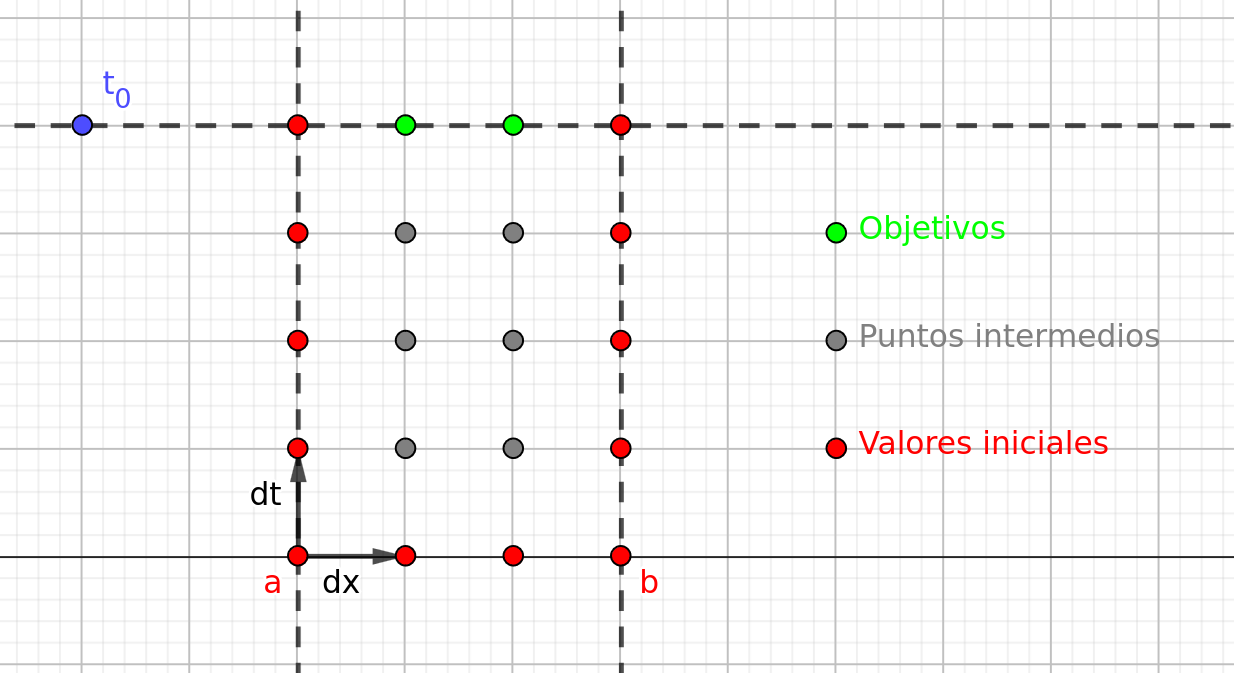
\includegraphics[scale=0.25]{./Imagenes/Bitmap/1dheatpoints.png}
	\caption{Representación en la malla del esquema \eqref{eq:1dheat_formula}}
	\label{fig:1d_grid}
\end{figure}

Antes de estudiar la convergencia de \eqref{eq:1dheat_formula}, presentamos el siguiente lema:

\begin{lema}
	Suponiendo que $u$ es suficientemente diferenciable, se tiene que
	\begin{equation}
		\label{eq:lema1_eq1}
		u^t(x,t)-u^{x,\bar{x}}(x,t) = \tau(x,t),
	\end{equation}
	donde $t$ es el error de truncamiento, definido como
	\begin{equation}
		\label{eq:lema1_eq2}
		\tau(x,t) = \frac{\Delta t}{2}\frac{\partial^2 u}{\partial t^2} + \frac{\Delta x^2}{12}\frac{\partial^4u}{\partial x^4} + \xi_{\Delta x, \Delta t}.
	\end{equation}
	Siendo $\xi_{\Delta x, \Delta t}$ un número real que cumple que
	\begin{equation}
		\xi_{\Delta x, \Delta t} \xrightarrow[\Delta x \rightarrow 0, \Delta t\rightarrow 0]{} 0 
	\end{equation}
	
\end{lema}

\begin{proof}
	Haciendo el desarrollo de Taylor de orden 2 para la función $u$ con centro en el punto $(x,t)$ tenemos
	\begin{multline}
		u(x,t+\Delta t)=u(x,t) + \frac{\partial u}{\partial t}\Delta t + \frac{1}{2}\frac{\partial^2u}{\partial t^2}\Delta t^2 + \xi^1_{\Delta x, \Delta t}\Delta t^2 \Rightarrow \\
		u^t(x,t) = \frac{\partial u}{\partial t} + \frac{\Delta t^2}{2}\frac{\partial^2u}{\partial t^2}\Delta t + \xi_{\Delta x, \Delta t}^1\Delta t,
	\end{multline}
	siendo $\xi^1_{\Delta x,\Delta t}$ un número que cumple la propiedad que le pedimos a $\xi_{\Delta x,\Delta t}$.
	
	Si nos fijamos en la igualdad resultante, la parte izquierda es exactamente el sumando izquierdo de \eqref{eq:lema1_eq1}, y la parte derecha es el primer sumando de \eqref{eq:lema1_eq2} más los términos $\frac{\partial u}{\partial t}$ y $\xi^1_{\Delta x, \Delta t}$.
	
	Si ahora hacemos los desarrollos de Taylor de orden 4 para la misma función y el mismo centro pero en otros puntos, obtenemos
	\begin{multline}\label{eq:lema1_eq3}
		u(x+\Delta x,t)= \\ u(x,t)+\frac{\partial u}{\partial x}\Delta x+\frac{1}{2!}\frac{\partial^2 u}{\partial x^2}\Delta x^2 + \frac{1}{3!}\frac{\partial^3u}{\partial x^3}\Delta x^3+\frac{1}{4!}\frac{\partial^4u}{\partial x^4}\Delta x^4 + \xi_{\Delta x, \Delta t}^2\Delta x^4
	\end{multline}
	y
	\begin{multline}
		u(x-\Delta x,t)= \\ u(x,t)-\frac{\partial u}{\partial x}\Delta x+\frac{1}{2!}\frac{\partial^2 u}{\partial x^2}\Delta x^2 - \frac{1}{3!}\frac{\partial^3u}{\partial x^3}\Delta x^3+\frac{1}{4!}\frac{\partial^4u}{\partial x^4}\Delta x^4 + \xi_{\Delta x, \Delta t}^3\Delta x^4
	\end{multline}
	siendo $\xi_{\Delta x, \Delta t}^2$ y $\xi_{\Delta x, \Delta t}^3$ números que cumplen la propiedad que le pedimos a $\xi_{\Delta x, \Delta t}$.
	Ahora, si sumamos las dos últimas ecuaciones, ya que se nos cancelan los términos con exponente impar, obtenemos
	\begin{equation}\label{eq:lema1_eq4}
		u^{x,\bar{x}} - \frac{\partial^2u}{\partial x^2}=\frac{1}{12}\frac{\partial^2u}{\partial x}\Delta x^2 + (\xi_{\Delta x, \Delta t}^2+\xi_{\Delta x, \Delta t}^3)\Delta x^2.
	\end{equation}

	Si restamos \eqref{eq:lema1_eq3} y \eqref{eq:lema1_eq4} (teniendo en cuenta que $\frac{\partial u}{\partial t} - \frac{\partial^2u}{\partial x^2}=0$) obtenemos precisamente la igualdad \eqref{eq:lema1_eq1}, siendo $\xi_{\Delta x, \Delta t} = \xi_{\Delta x, \Delta t}^1\Delta t - (\xi_{\Delta x, \Delta t}^2+\xi_{\Delta x, \Delta t}^3)\Delta x^2$, por lo que se confirma que tiende a 0 cuando los incrementos tienden a 0.
\end{proof}

\begin{teorema}
	Si $0<\lambda<\frac{1}{2}$, el método numérico \eqref{eq:1dheat_formula} es convergente\footnote{De hecho, el método converge si y solo si $0<\lambda<\frac{1}{2}$, pero no lo probaremos por que solo nos interesa cuado converge}, o dicho de otra forma, si definimos el error de aproximación del método $\epsilon_{i,j}:=|u_{i,j}-U_{i,j}|$, $\sup_{i,j}\epsilon(i,j)\rightarrow0$ si $\Delta t, \Delta x \rightarrow 0$.
\end{teorema}



\begin{proof}
	Teniendo en cuenta el lema anterior, si ahora repetimos las cuentas que nos llevaron a \eqref{eq:1dheat_formula} pero para $u$ en lugar de para $U$, obtenemos la ecuación
	\begin{equation}
		u_{i,j+1} = (1-2\lambda)u_{i,j}+\lambda(u_{i-1,j}+u_{i+1,j})+\Delta t\tau_{i,j},
	\end{equation}
	por lo que
	\begin{gather}
		\epsilon_{i,j+1} = |u_{i,j+1}-U_{i,j+1}| = \\ |((1-2\lambda)u_{i,j}++\lambda(u_{i-1,j}+u_{i+1,j})+\Delta t\tau_{i,j}) \\
		 - ((1-2\lambda)U_{i,j}++\lambda(U_{i-1,j}+U_{i+1,j}))| = \\
		 |(1-2\lambda)(u_{i,j}-U_{i,j})+\lambda(u_{i+1,j}-U_{i+1,j}+u_{i-1,j}-U_{i-1,j}) + \Delta t\tau_{i,j}|.
	\end{gather}
	Utilizando la desigualdad triangular, obtenemos
	\begin{multline}
		\epsilon_{i,j+1} \leq (1-2\lambda)|u_{i,j}-U_{i,j}|+\lambda(|u_{i+1,j}-U_{i+1,j}|+|u_{i-1,j}-U_{i-1,j}|) + \Delta t|\tau_{i,j}| \\
		= (1-2\lambda)\epsilon_{i,j}+\lambda(\epsilon_{i+1,j}+\epsilon_{i-1,j}) + \Delta t|\tau_{i,j}|.
	\end{multline}
	Ahora, si definimos
	\begin{equation}
		E_j:=\sup_{i}|\epsilon_{i,j}|\hspace{30px}\tau:=\sup_{i,j}|\tau_{i,j}|
	\end{equation}
	tenemos que
	\begin{equation}
		E_{j+1}\leq E_j+\Delta t\tau,
	\end{equation}
	mediante una inducción trivial concluimos que
	\begin{equation}
		E_j \leq E_0 + j\Delta t\tau = E_0+t_j\tau = t_j\tau,\hspace{15px}\forall j\geq0
	\end{equation}
	donde $E_0$ es el supremo del error en $t=0$ (que es $0$ porque $U_{i,0} =f(x_i)= u_{i,0}$ por definición).
	
	Con esto hemnos acabado la demostración, pues está claro (por su definición) que $\tau$ tiende a 0 cuando $\Delta t, \Delta x$ tienden a 0, luego el error está acotado por algo que tiende a 0, lo que implica que tiende a 0.
\end{proof}

\section{Caso bidimensional}

En el caso bidimensional, la ecuación que tenemos será
\begin{equation}\label{eq:2dheat}
	\frac{\partial u}{\partial t}=\frac{\partial^2u}{\partial x^2}+\frac{\partial^2u}{\partial y^2}
\end{equation}

\com{Voy a dejar esto en stand by, estoy teniendo problemas para encontrar algún teorema de existencia y unicidad para alguna condición inicial, y por tanto no sé que condiciones iniciales voy a acabar pidiéndole.}




